\documentclass{article}

% if you need to pass options to natbib, use, e.g.:
% \PassOptionsToPackage{numbers, compress}{natbib}
% before loading nips_2016
%
% to avoid loading the natbib package, add option nonatbib:
% \usepackage[nonatbib]{nips_2016}

\PassOptionsToPackage{numbers,sort&compress}{natbib}
\usepackage[final]{nips_2016} % produce camera-ready copy

\usepackage[utf8]{inputenc} % allow utf-8 input
\usepackage[T1]{fontenc}    % use 8-bit T1 fonts
\usepackage{hyperref}       % hyperlinks
\usepackage{url}            % simple URL typesetting
\usepackage{booktabs}       % professional-quality tables
\usepackage{amsfonts}       % blackboard math symbols
\usepackage{nicefrac}       % compact symbols for 1/2, etc.
\usepackage{microtype} 
\usepackage{graphicx} % microtypography
\usepackage{amsmath} 
\usepackage{multirow}
\usepackage{appendix}
\usepackage{float}
\usepackage{booktabs}
\usepackage{xcolor}
\usepackage{subcaption}
\usepackage{hyperref}
\hypersetup{
    colorlinks=true,
    urlcolor=blue
}

% Reduce paragraph spacing
\setlength{\parskip}{3pt}

% Widen abstract
\renewenvironment{abstract}
  {\small
   \begin{center}
   \bfseries \abstractname\vspace{-.5em}\vspace{0pt}
   \end{center}
   \list{}{%
     \setlength{\leftmargin}{0.5cm}% Reduced left margin
     \setlength{\rightmargin}{\leftmargin}% Match right margin
   }%
   \item\relax}
  {\endlist}

\title{Unveiling the Dynamics of Music Popularity on Spotify:
 Temporal Trends and Popularity Drivers}

\begin{document}

\maketitle

 % Reduce space between title and abstract

\begin{abstract}
The rapid expansion of music streaming platforms and increasing competition among various platforms  has created a vast opportunity to understand the track popularity, artist success, and popular songs. We operate as skunkworks team within Spotify investigating the Top 200 global chart dataset (2017 – 2023) consisting of audio features, artist metadata and popularity metrics. Through exploratory data analysis, we examine temporal streaming patterns across years, months, and weeks, while examining whether it's the artist or song audio features that drives the success of the track. We build Random forest, Logistic Regression, SVM, and XGBoost models with accuracies ranging from 50-70\%. Our findings contribute to music information retrieval (MIR) research by explaining how multi level feature aggregation improve forecasting in streaming environments, with future work exploring Graph Neural Networks for enhanced prediction in successful collaboration.
\end{abstract}

\vspace{-0.3cm} % Reduce space after abstract

\section{Introduction}

Digital streaming platforms like Spotify \cite{Spotify}, YouTube Music \cite{YouTubeMusicPlatform}, and Apple Music \cite{AppleMusic} have transformed music consumption, as they generate vast behavioral and acoustic data that fuels Hit Song Science (HSS) research \cite{schedl2016, oord2013}. While audio features such as energy, valence, and danceability correlate with popularity \cite{kim2020, pachet2008}, success is shaped by more than sound alone—cultural impact \cite{salganik2006}, collaboration networks \cite{herd2022, oliveira2020detecting}, and artist identity play critical roles \cite{macia2023}. Despite recognition of social media influence \cite{salganik2006} and collaboration patterns \cite{oliveira2020detecting}, very few studies integrate long-term global chart analysis with artist-level features and collaboration networks \cite{macia2023}.

We fix this by analyzing Spotify's Global Top 200 charts (2017–2023) through machine learning-driven exploratory analysis. Using audio features, time-aware artist metadata, and a points-based popularity metric, we investigate: \textbf{(1) Are there any temporal patterns in what day(s) of the week and/or months experience the most streams?} and \textbf{(2) Which factors, artist reputation or audio characteristics, drive song popularity?} Our approach uses evidence-based insights into the evolving dynamics of global music popularity.

% By combining exploratory analysis with predictive modeling, we evaluate how multi-level feature aggregation can meaningfully forecast success in the evolving global music landscape.

% ==================================================================
% ======================== OLD INTRODUCTION ========================
% ==================================================================
% Music consumption today is fundamentally different from what it was before digital streaming services became mainstream. Streaming platforms like Spotify, Apple Music, and YouTube provide enormous behavioral datasets that open up new avenues for research in music information retrieval, including hit prediction, audio-based modeling, and recommendation systems \citep{schedl2016, oord2013}. Early studies have demonstrated that measurable musical features can anticipate commercial success \citep{pachet2008}, while more recent work has identified acoustic properties such as energy, valence, loudness, and danceability that correlate with track popularity \citep{kim2020}. However, artist identity, collaboration networks, and cultural factors beyond song-level features also underpin global consumption patterns \citep{herd2022, macia2023}, and social influence can make popularity unpredictable \citep{salganik2006}. Despite this growing research, few works have combined temporal dynamics, track features, artist characteristics, and collaboration patterns within long-term global chart analysis, particularly examining how major disruptions like the COVID-19 pandemic reshaped streaming behaviors.

%\In this project, we operate as a skunkworks team within Spotify to investigate the Top 200 global charts dataset (2017-2023), containing 651,936 daily entries across 9,161 unique tracks from 2,208 artists, enriched with audio descriptions, artist metadata, and a points-based popularity scoring system. The study period spans three distinct eras: pre-pandemic (2017-2019), pandemic disruption (2020-2021), and recovery (2022-2023), allowing us to examine how streaming behaviors and collaboration patterns evolved through extraordinary circumstances. We focus majorly on exploratory data analysis to unveil temporal features across years, months, and weeks, while examining the determinants of popularity specifically whether chart success is mainly driven by song-level audio features or artist-level characteristics like reputation and historical performance. We then address a predictive challenge: can we identify which collaborations (particularly tracks with multiple artists) will break into the top-50 using machine learning? Focusing on the top-50 threshold balances commercial relevance with sufficient sample size for robust modeling. Using Logistic Regression as our best-performing classifier, we achieved 70.5\% accuracy, 77.57\% AUC, and 67.19\% recall in predicting successful collaborative hits for 2024, demonstrating that multi-level feature aggregation can meaningfully forecast streaming success.

\section{Data Preprocessing}
\subsection{Dataset Description}
This dataset contains Spotify Top 200 tracks from 2017-01-01 to 2023-05-29, and consists of 651,936 rows and 20 columns. Each track contains features like ranking position, points (popularity proxy) artist name, Nationality, and various Spotify audio features (Danceability, Energy, Loudness, Speechiness, Acousticness, Instrumentalness, and Valence) which we used for our analysis.


\subsection{Data Aggregation and Feature Scaling}
\begin{itemize}
    \item \textbf{Audio Feature Standardization}:* The audio feature - loudness ranged from -34,475 to 1,509 dB which is an extreme range that could dominate over the model and hence it was normalized by 1000. Post correction it ranged between -34.48 to 1.51 dB ensuring a balanced contribution.

    \item \textbf{Unique Song Aggregation}: * The original dataset contained entries (651,936 rows) comprising multi-row-per-song due to artist collaboration. To transform this into a unique song dataset to preserve meaningful information while eliminating redundancy, we aggregated all the features and grouped them by the song id.

\end{itemize}

\subsection{Target Variable Engineering}
In order to investigate what drives popularity of the song, we need a robust measure of success and so we created a 3-class target variable using percentile-based threshold

\begin{table}[h!]
\centering
\begin{tabular}{|c|c|c|c|}
\hline
\textbf{Success Class} & \textbf{Threshold Points} & \textbf{Percentage of Songs} & \textbf{Distribution} \\
\hline
Low & $\leq$ 2,901 & 70.0\% & 6,413 songs \\
\hline
Moderate & 2,901 - 19,884 & 20.0\% & 1,832 songs \\
\hline
Hit & $>$ 19,884 & 10.0\% & 916 songs \\
\hline
\end{tabular}
\vspace*{0.2cm}
\caption{Target Variable Classification Based on Accumulated Chart Points}
\label{tab:target_variable}
\end{table}

% \vspace*{-0.3cm}
The thresholds stated in Table ~\ref{tab:target_variable} are based on the 70th percentile at 2,901 points and 90th percentile at 19,884 points of the points distribution; this would result in balanced classes, reflecting real-world music success patterns but still having enough samples to drive robust modeling.
The final classification achieved near exact proportional splits (70.0\% / 20.0\% / 10.0\%) matching our percentile-based design goals.


\subsection{Time-Aware Artist Feature Engineering}
The features  mentioned in ~\ref{tab:artist_features} were calculated to interpret the artist historical performance before the song release. For each song released at time t, we can calculated:

\begin{table}[h!]
\begin{tabular}{|c|c|c|}
\hline
\textbf{Feature} & \textbf{Calculation} & \textbf{Interpretation} \\
\hline
Artist\_Past\_Avg\_Points & mean(points before $t$) & Historical performance baseline \\
\hline
Artist\_Past\_Max\_Points & max(points before $t$) & Peak capability indicator \\
\hline
Artist\_Experience & count(songs before $t$) & Career longevity measure \\
\hline
Artist\_Days\_Since\_Last & $t$ - max(dates before $t$) & Release frequency pattern \\
\hline
Is\_Debut & 1 if no previous songs, else 0 & First-release effect \\
\hline
\end{tabular}
\centering
\vspace*{0.2cm}
\caption{Time-Aware Artist Feature Engineering}
\label{tab:artist_features}
\end{table}

\vspace*{-0.7cm}
\subsection{Collaboration Dynamics}
The features listed in ~\ref{tab:collaboration_features} were created as they  directly address whether popularity is determined by combined artists and audience groups, testing whether collaborative efforts produce a multiplicative rather than an additive success effect

\begin{table}[h!]
\footnotesize
\begin{tabular}{|p{2.0cm}|p{3.0cm}|p{7.5cm}|}
\hline
\textbf{Feature} & \textbf{Description} & \textbf{Purpose} \\
\hline
Is\_Collaboration & Binary flag (1 if multiple artists, 0 if solo) & Tests synergistic effects: whether artist combinations create popularity beyond individual capabilities \\
\hline
Num\_Artists & Count of contributing artists per song & Measures network size impact: whether more artists correlate with increased audience reach \\
\hline
\end{tabular}
\vspace*{0.2cm}
\centering
\caption{Collaboration Feature Engineering}
\label{tab:collaboration_features}
\end{table}

\vspace{-0.5cm}
\section{Exploratory Data Analysis}
\subsection{Univariate Analysis}

We examined the distribution of all audio and artist features to understand their statistical properties and identify patterns relevant to modeling.

\begin{figure}[!htb]  
    \centering
    
    % Left: Audio Features
    \begin{subfigure}[c]{0.49\textwidth}  
        \centering
        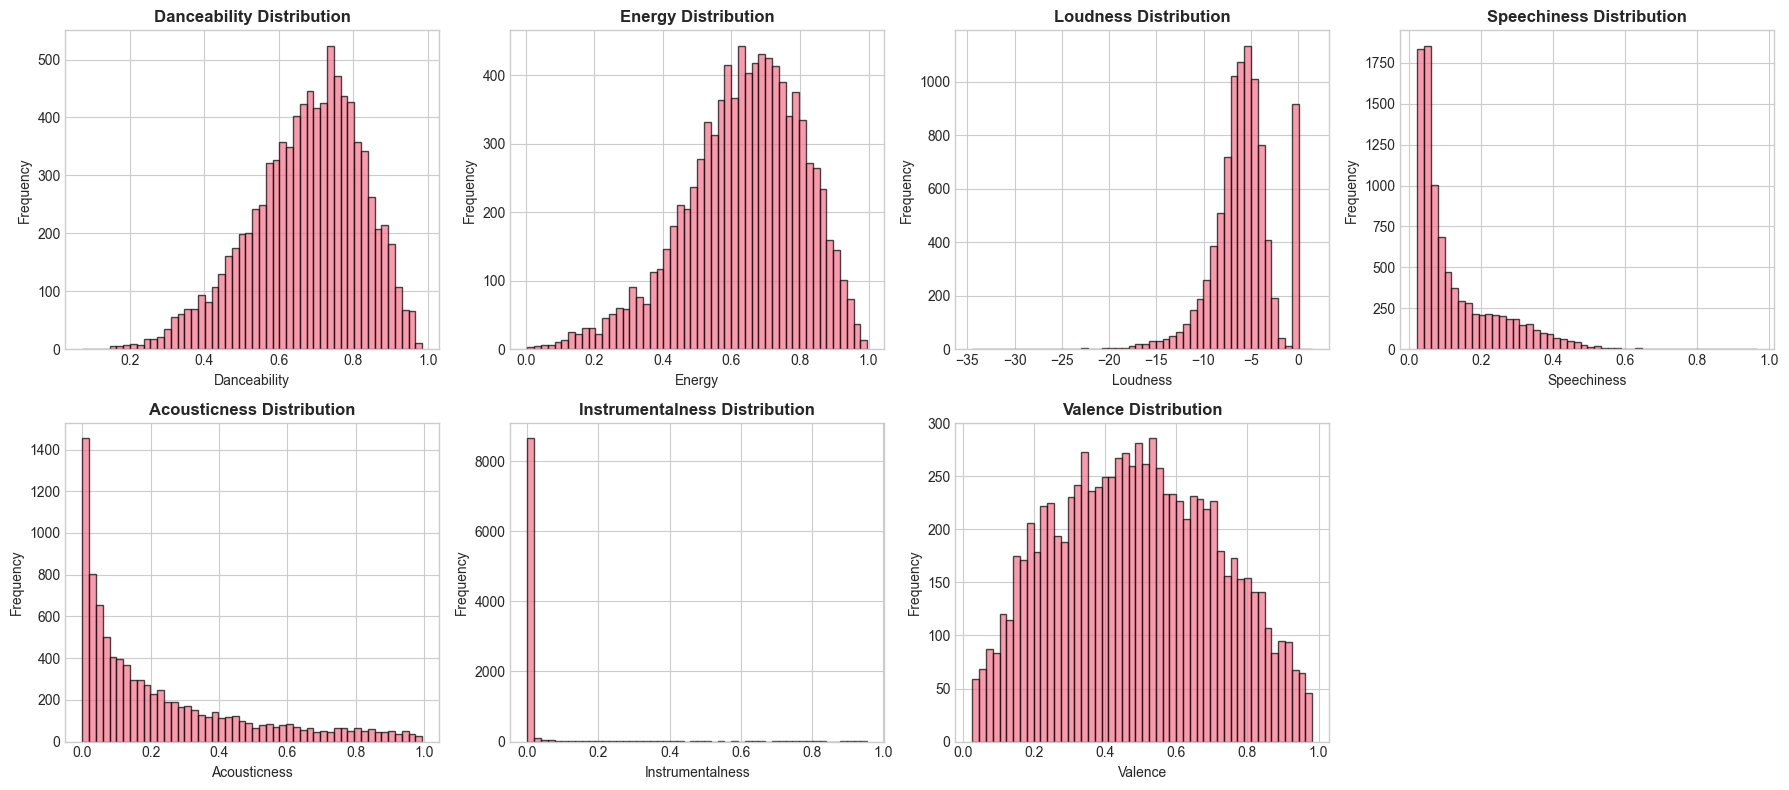
\includegraphics[width=\textwidth, height=6cm, keepaspectratio]{figs/uni_audio.png}
        \vspace{0.1cm}
        
        \caption{Audio Features}  
        \label{fig:univariate audio}  
    \end{subfigure}
    \hfill
    % Right: Artist Features  
    \begin{subfigure}[c]{0.49\textwidth} 
        \centering
        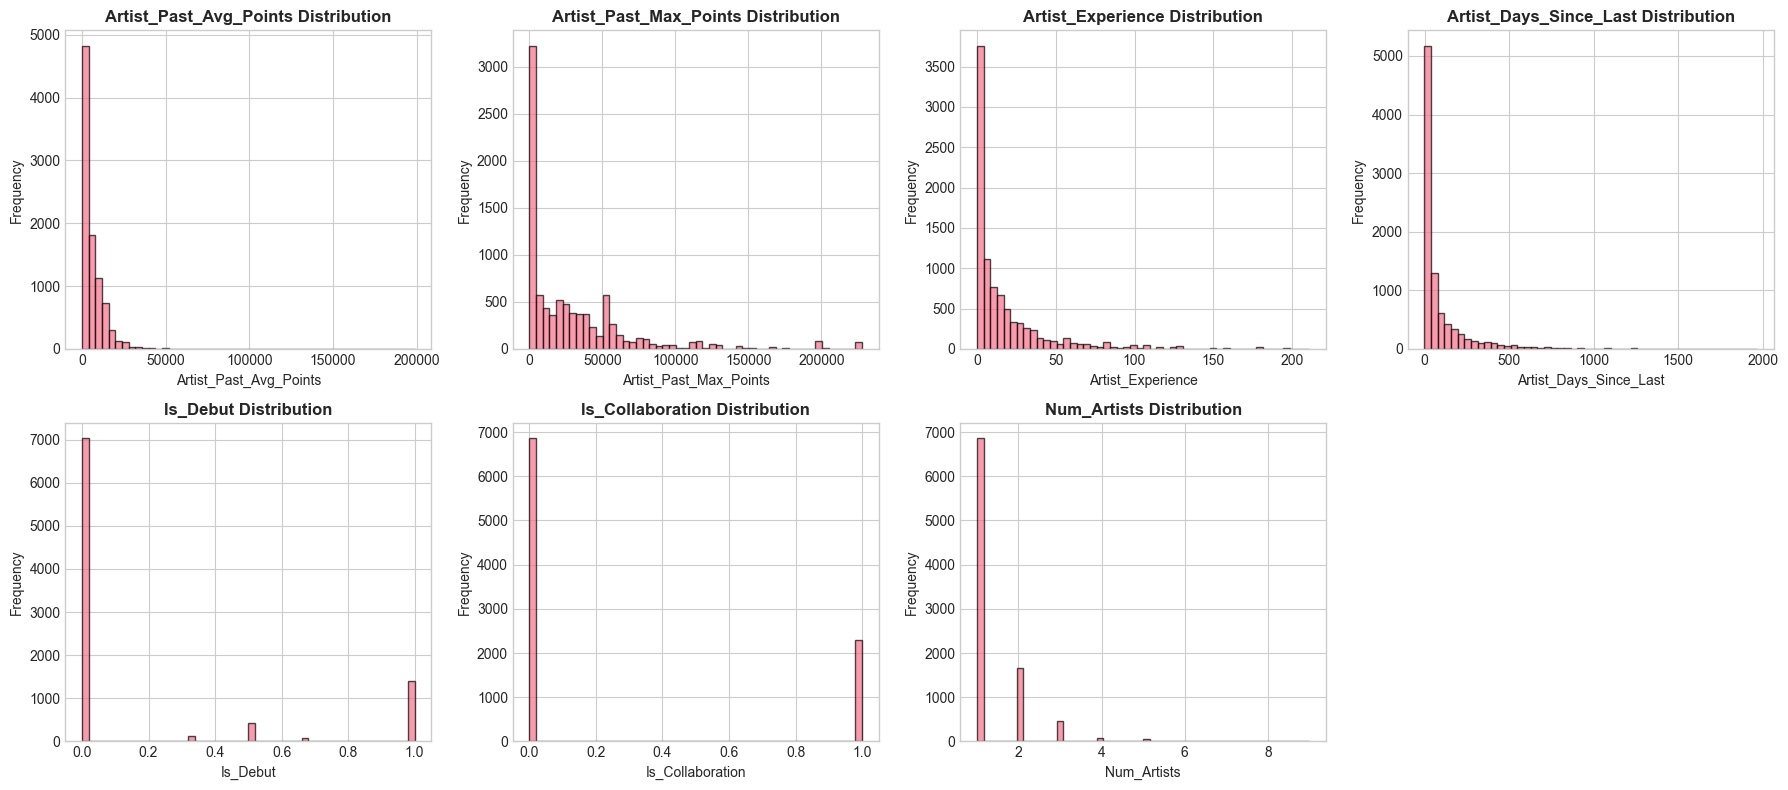
\includegraphics[width=\textwidth, height=6cm, keepaspectratio]{figs/uni_artist.png}
        \vspace{0.1cm}
        
        \caption{Artist Features}  
        \label{fig:univariate artist}
    \end{subfigure}
    
    \caption{Univariate analysis of Audio features and Artist Features}
    \label{fig:univariate}
\end{figure}

Figure ~\ref{fig:univariate audio} shows the distribution of audio features: Danceability ($\mu$=0.67), Energy ($\mu$=0.64), Loudness ($\mu$=–5.82 dB), Valence ($\mu$=0.49) have a \textbf{Normal Distribution}, good for parametric models while Speechiness (Mdn=0.08) \& Acousticness (Mdn=0.14)  have a ~\textbf{Right-skewed distribution}, showing dominance of vocal electronic tracks. Instrumentalness is heavily concentrated at 0 (75th percentile = 0), almost all charting songs are vocal.

Figure ~\ref{fig:univariate artist} show the distribution of all the  artist features. the Features Artist\_Past\_Avg\_Points (Mdn=3,459 vs Mean=5,784) and Artist\_Past\_Max\_Points (Mdn=18,127 vs Mean=29,859) have a very strong ~\textbf{Right Skew Distribution}. Artist\_Experience has a Mdn=7, Artist\_Days\_Since\_Last Release has a Mdn=28 indicating active but not highly prolific artists. There is a 80.8\% non-debut artists and 25.1\% collaborations.

\vspace{-.1cm}
\subsection{Bivariate Distribution}
The Bivariate analysis tests our hypothesis of which either the audio properties or artist reputation have stronger associations with success by examining how each of them correlate with the target feature - success class, thereby identifying which of them discriminate between the class low, moderate and High. 
\begin{figure}[!htb]
    \centering
    
    % Left: Audio Features
    \begin{subfigure}[t]{0.49\textwidth}
        \centering
        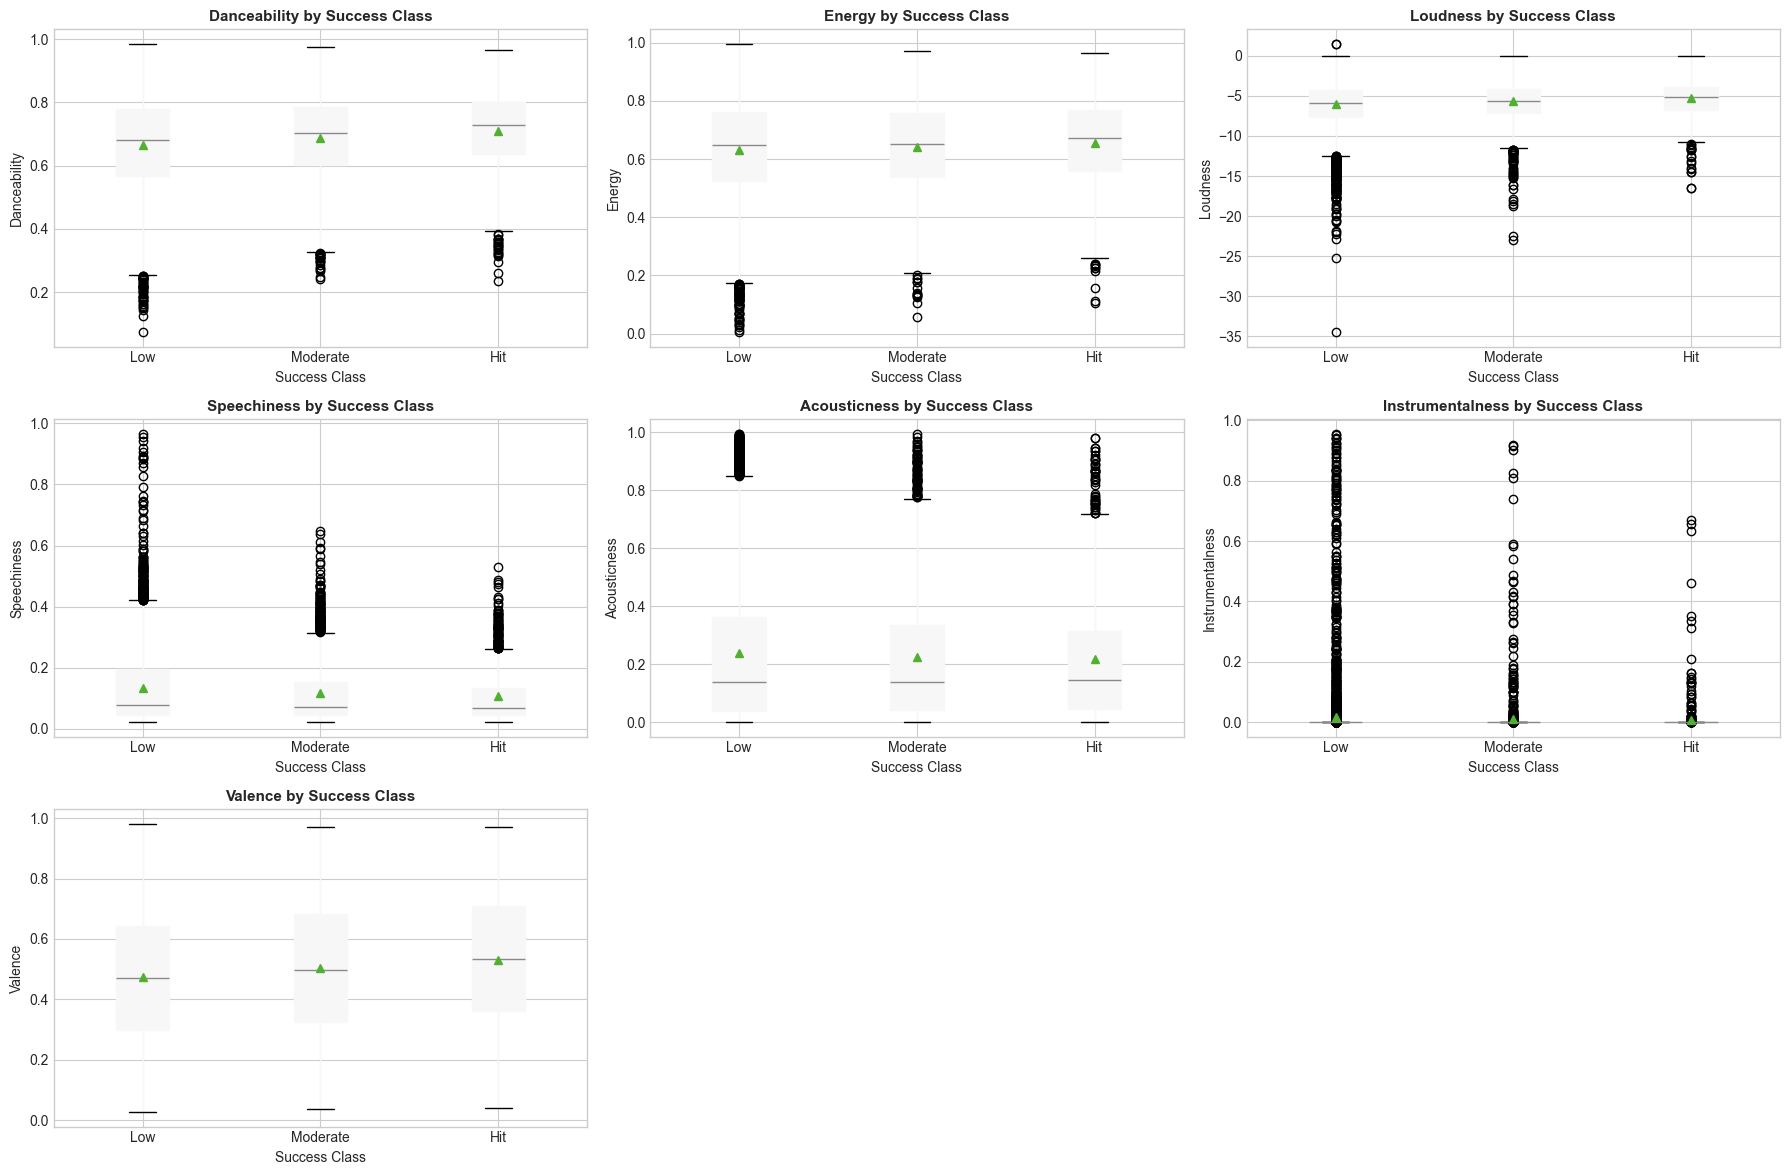
\includegraphics[width=\textwidth]{figs/multi_audio.png}
        \caption{Audio Features by Target Class}
        \label{fig:multi_audio}
    \end{subfigure}%
    \hfill
    % Right: Artist Features  
    \begin{subfigure}[t]{0.49\textwidth}
        \centering
        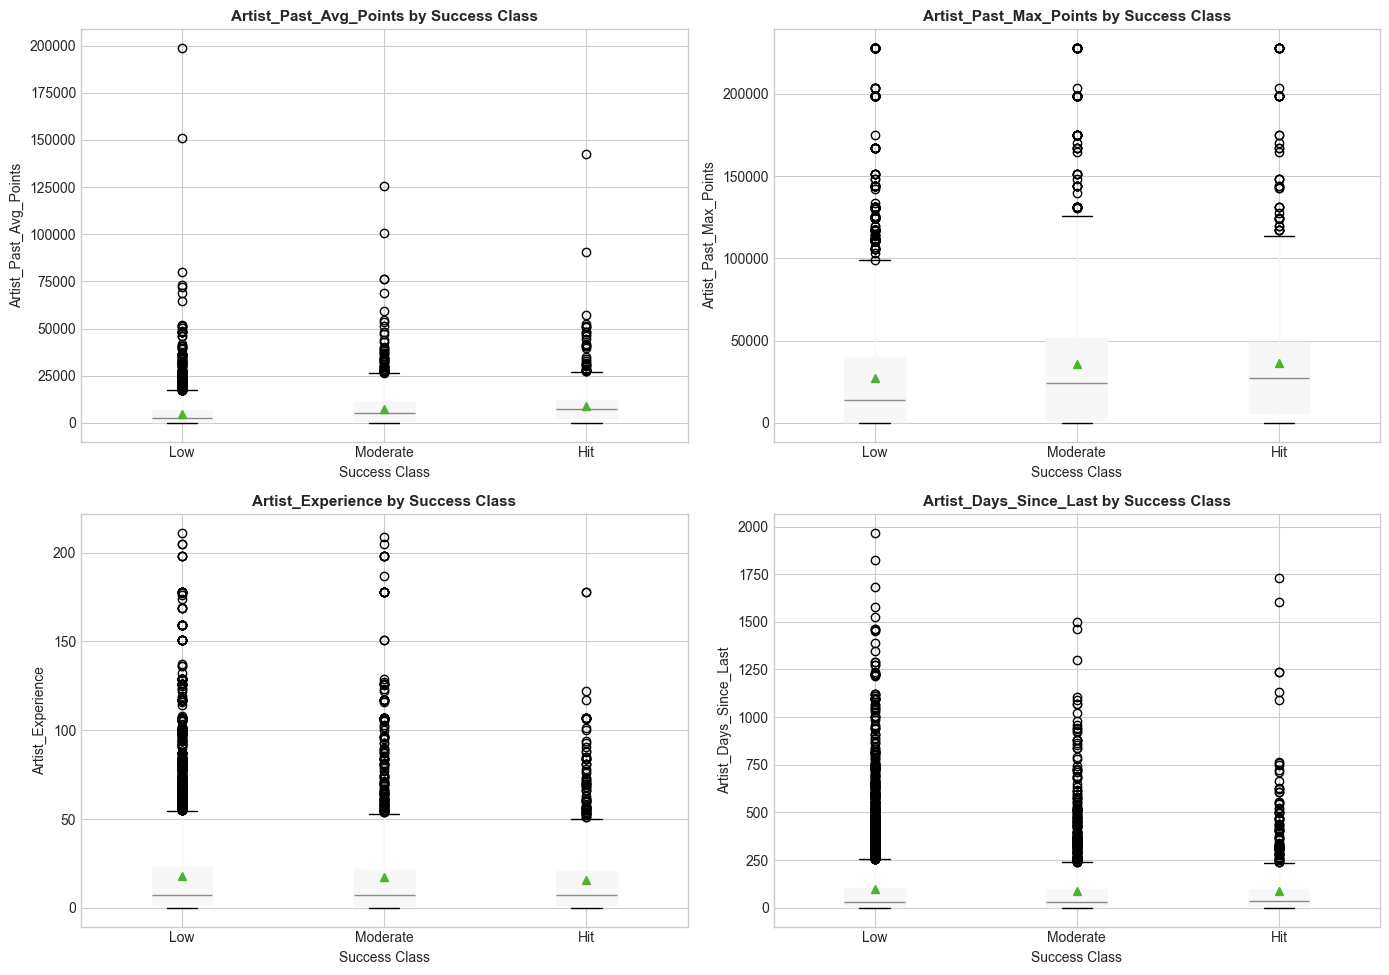
\includegraphics[width=\textwidth]{figs/multi_artist.png}
        \caption{Artist Features by Target Class}
        \label{fig:multi_artist}
    \end{subfigure}
    
    \caption{Bivariate analysis: Feature distributions across success classes (Low/Moderate/Hit)}
    \label{fig:bivariate}
\end{figure}

The Audio features in Figure ~\ref{fig:multi_audio} (Appendix) show Hits only show modest lifts: Danceability (+6.5\%); Energy (+3.8\%); Loudness (+13\%, +0.76 dB); and Valence (+12\%). Speechiness, Acousticness, and Instrumentalness are slightly lower. But heavy IQR overlap meaning the audio traits barely separate Low vs. Hit songs reflecting mastering norms more than creative differences.

 Figure ~\ref{fig:multi_artist} (Appendix) shows the Artist Features emerging as the most potent predictors of success. Hit songs are from artists with much stronger track records, as demonstrated by the 86.8\% increase in Artist\_Past\_Avg\_Points ($\mu$=4,855 → $\mu$=9,068) and a 35\% increase in Artist\_Past\_Max\_Points. This increase suggests that selective, high-quality output is more important than volume, as indicated by the decrease in Artist\_Experience by 13.1\%. Artists releasing slightly more frequently fare better, as demonstrated by an 8.4\% drop in Days\_Since\_Last. %Collaboration is the strongest binary indicator, with 49.5\% of hits being collaborations compared to 20.3\% for low-performing songs-a 2.4× advantage.

 \subsection{Correlation Matrix}

The results of the correlation analysis ~\ref{fig:correlation_heatmap} (Appendix) are particularly critical to our approach to modeling. Strong inter-feature correlations, especially those between Energy and Loudness at 0.56, and among artist historical metrics, such as Artist\_Past\_Avg\_Points and Artist\_Past\_Max\_Points at 0.59, point to significant feature redundancy that calls for dimensionality reduction. More importantly, the weak correlations with our target variable-the fact that no audio feature exceeds 0.33 for Valence and the artist metrics show only modest relationships, with Artist\_Past\_Avg\_Points at 0.14-no single feature is dominating predictive power. This directly supports our ensemble modeling strategy and explains the consistent advantages seen in our experiments, where artist-based features tend to always outperform those that are audio-only.

\section{Temporal Analysis}

\subsection{Temporal Streaming Trends}
Figure ~\ref{fig:YoY_avg_points} and Table ~\ref{tab:temporal_stats} tells us how global events and platform evolution reshaped music consumption patterns during 2017 to 2023. But we excluded 2023 data from temporal analysis since it only contains five months. We use points as a measure of streaming activity. 
\begin{figure}[!ht]
    \centering
    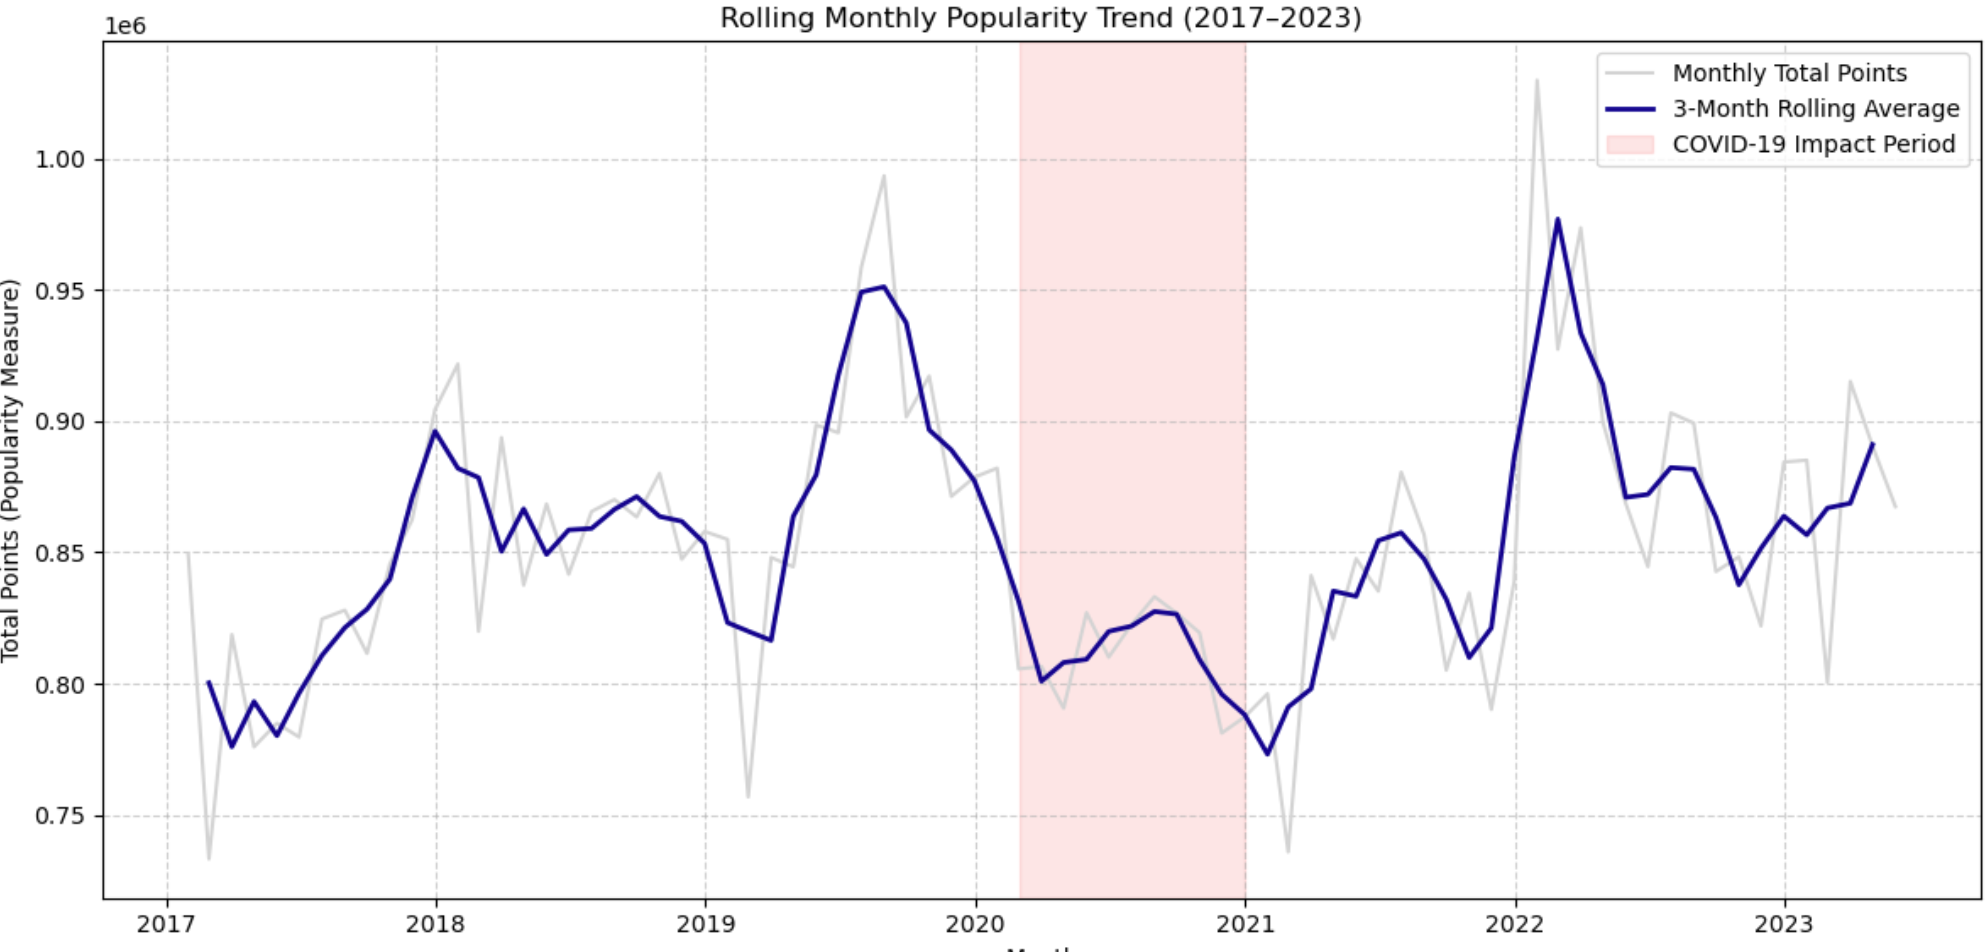
\includegraphics[width=0.6\linewidth]{figs/YoY_points_avg.png}
    \caption{Year-over-Year Average Streaming Points Trend Affected by COVID-19}
    \label{fig:YoY_avg_points}
\end{figure}



\begin{table}[h]
\begin{tabular}{|c|c|c|c|c|}
\hline
\textbf{Year} & \textbf{Total Points} & \textbf{Unique Songs} & \textbf{Collab \%} & \textbf{Longevity (Days)} \\ \hline
2017 & 9,818,064 & 1,551 & 24.89\% & 72.9 \\ \hline
2018 & 10,368,011 & 1,924 & 29.11\% & 53.6 \\ \hline
2019 & 10,619,250 & 1,765 & 30.55\% & 53.1 \\ \hline
2020 & 9,792,540 & 2,004 & 25.37\% & 42.3 \\ \hline
2021 & 9,879,331 & 1,822 & 24.34\% & 42.2 \\ \hline
2022 & 10,743,685 & 1,589 & 31.08\% & 32.0 \\ \hline
\end{tabular}
\centering
\vspace{0.3cm}
\caption{Comprehensive temporal statistics showing pandemic disruption across metrics}
\label{tab:temporal_stats}
\end{table}




\begin{itemize}
    \item \textbf{Pre-Pandemic Growth (2017–2019)}: Steady growth to 10.62M points in 2019, driven by platform expansion and rising global adoption.\cite{hansen2022musicspending}
    \item \textbf{COVID-19 Disruption (2020)}: Sharp 7.8\% drop in 2020 (total points),the dataset's sharpest decline, as lockdowns cut commute listening\cite{aguiar2021covid}; collaborations fell from 30.55\% → 25.37\% (Table~\ref{tab:temporal_stats}). Podcasts diverted the attention from music to podcast during this phase indicating due to pandemic restrictions in person studio collaborations were limited collaborations.\cite{spotify_podcast_expansion_2020}
    \item \textbf{Sluggish Recovery (2021)}: Minimal rebound (+0.9\%) was observed despite vaccines coming out for covid, and adoption of remote work and podcast persisted.\cite{ye2022variety}
    \item \textbf{Post-Pandemic Surge (2022)}: Streaming jumped 8.8\% to 10.74M (Table~\ref{tab:temporal_stats}), fueled by return-to-office and increased the  demand for live music.\cite{hansen2022musicspending}
    \item \textbf{Accelerating Consumption Cycles}: Song chart longevity collapsed 56\%—from 73 days (2017) to 32 days (2022)—driven by TikTok's viral mechanics. Songs now spike rapidly through social media trends but fade quickly, fundamentally shortening the "hit lifespan." This reflects algorithmic discovery replacing traditional radio-driven slow-burn hits.\cite{ye2022variety}
    \item \textbf{Weekday Patterns}: Weekend engagement peaks at +2.2\% (Saturday, Table~\ref{tab:weekday_patterns}) above weekly average, consistent with leisure-time listening replacing work/commute consumption.\cite{krause2022covidlistening}
\end{itemize}

\subsection{Consumption Timing: Weekday and Monthly Patterns}
The table \ref{tab:weekday_patterns} shows us the streaming patterns by day of weeks shows consistent weekend effects. Saturday has the highest streaming points( 8,888,057 total points) 2.2\% higher than weekdays average. Sunday show’s the second most highest streaming points with +0.6\% higher relative average then normal days, while Monday to Thursdays’ the streams remain relatively stable showed a relatively low average than weekdays varying between 0\% and -0.5\% . Streaming increases from Fridays on Spotify we can easily see the relative difference between the weekdays and weekends pattern. Monthly patterns \ref{tab:monthly_patterns} shows that December being the highest ranking streaming months due to holiday and festival season. In mid year summer months also shows elevated engagement between(July – August). February typically indicates lowest monthly total points.January 2022 shows great performance (10,381 average points), possibly due to post holidays consumption. These temporal insights provide the strategic insights for release timing, with weekend releases and specific months offering potential advantages.

\vspace{-0.2cm}
\section{Learning Methodologies}
\subsection{Methodology Overview}
In order to assess whether the artist reputation or the audio characteristics drive the popularity of a song, we employed a comparative modeling framework using four different machine learning algorithms across three models - Audio Only (Danceability, Energy, Loudness, Speechiness, Acousticness, Instrumentalness, Valence); Artist Only (Artist\_Past\_Avg\_Points, Artist\_Past\_Max\_Points, Artist\_Experience, Artist\_Days\_Since\_Last', Is\_Debut, Is\_Collaboration, Num\_Artists); and Combined (Audio Features + Artist Features). This multi-algorithm approach was used to ensure that our findings are robust across the different learning paradigms and not artifacts of one single model.

\subsection{Algorithm Selection \& Rationale}
The following four algorithms ~\ref{tab:algorithms} were selected representing distinct paradigms to ensure an intricate coverage. 

\begin{table}[h!]
\begin{tabular}{|p{3cm}|p{10cm}|}
\hline
\textbf{Algorithm} & \textbf{Rationale \& Learning Paradigm} \\
\hline
Random Forest \cite{RandomForest} & Ensemble tree-based learner \cite{ensemble_techniques} powerful to treat the outliers and non-linear relationships. It handles all the  imbalanced classes well and provides interpretable feature importance. \\
\hline
Logistic Regression \cite{LogisticRegression} & Linear baseline model with comprehensible coefficients. It tests whether the relationships are fundamentally linear or require non-linear modeling. \\
\hline
XGBoost \cite{GradBoost} & State-of-the-art gradient boosting algorithm. It is benchmark for structured data, excels with complex feature interactions and class imbalance. \\
\hline
Support Vector Machine \cite{SupportVecMach} & Margin-based learner using kernel methods (RBF). It tests the class separability in high-dimensional transformed space. \\
\hline
\end{tabular}
\vspace{0.2 cm}
\centering
\caption{Algorithm Selection Rationale and Learning Paradigms}
\label{tab:algorithms}
\end{table}

\subsection{Evaluation Strategy and Metrics}
The data was split as 80/20 test-train with propotional sampling maintaining the class distribution (70\%-Low, 20\%-Moderate, 10\%-Hit). A 5-fold stratified Cross-Validation was chosen over a single split due to: (1) reduces variation in measurement of performance, (2) provides a strong evaluation across the multiple data partition, (3) stratification preserves the class balance. This was performed only on the training set in order to prevent any data leakage. The metrics used were: (1) Accuracy - overall correctness; (2) Weighted F1-Score - harmonic mean of precision/recall weighted by class support, addresssing all the imbalance. Feature Scaling was also performed: StandardScalar was applied to Linear Regression(distance-based) and Support Vector Machine(scale-sensitive); the tree-methods use raw features(scale-variant). 

\subsection{Hyperparameter Tuning Strategy}
Hyperparameters \ref{tab: Hyperparameter_search_space_for_models} (Appendix) were selected to: (1) prevent overfitting (dataset: 9,161 songs), (2) handle class imbalance (70-20-10). All algorithms used class\_weight='balanced'. Tree models: max\_depth=6-10, n\_estimators=100. LR: multinomial solver. SVM: RBF kernel, C=1.0. XGBoost: learning\_rate=0.1. Values from preliminary grid search. Artist superiority across all configurations confirms finding is not hyperparameter-dependent.

\section{Results}

% \begin{table}[h!]
% \renewcommand{\arraystretch}{1.5} % Increased row spacing
% \begin{tabular}{|l|l|r|r|r|}
% \hline
% \textbf{Algorithm} & \textbf{Feature Set} & \textbf{Test Accuracy} & \textbf{Test F1-Score(Weighted)} & \textbf{Gap} \\
% \hline
% \multirow{3}{*}{Random Forest} 
%     & Audio Only & 51.9\% & 0.550 & \\
%     \cline{2-5}
%     & \textbf{Artist Only} & \textbf{53.0\%} & \textbf{0.567} & \textbf{+1.1pp} \\
%     \cline{2-5}
%     & Combined & 59.1\% & 0.616 & \\
% \hline
% \multirow{3}{*}{Logistic Regression}
%     & Audio Only & 43.6\% & 0.476 & \\
%     \cline{2-5}
%     & \textbf{Artist Only} & \textbf{51.3\%} & \textbf{0.549} & \textbf{+7.7pp} \\
%     \cline{2-5}
%     & Combined & 53.8\% & 0.570 & \\
% \hline
% \multirow{3}{*}{XGBoost}
%     & Audio Only & 69.6\% & 0.579 & \\
%     \cline{2-5}
%     & \textbf{Artist Only} & \textbf{70.0\%} & \textbf{0.628} & \textbf{+0.4pp} \\
%     \cline{2-5}
%     & Combined & 69.9\% & 0.626 & \\
% \hline
% \multirow{3}{*}{SVM}
%     & Audio Only & 40.7\% & 0.457 & \\
%     \cline{2-5}
%     & \textbf{Artist Only} & \textbf{49.9\%} & \textbf{0.539} & \textbf{+9.2pp} \\
%     \cline{2-5}
%     & Combined & 52.0\% & 0.560 & \\
% \hline
% \end{tabular}
% \vspace{0.2cm}
% \centering
% \caption{Algorithm Performance Comparison Across Feature Sets}
% \label{tab:algorithm_performance}
% \end{table}


% ==============================================
\begin{table}[h!]
\centering
\footnotesize
\setlength{\tabcolsep}{6pt}
\renewcommand{\arraystretch}{1.25}

\begin{tabular}{lcccccc}
\hline
& \multicolumn{2}{c}{\textbf{Audio}} 
& \multicolumn{2}{c}{\textbf{Artist}} 
& \multicolumn{2}{c}{\textbf{Combined}} \\
\hline
\textbf{Algorithm} 
& \textbf{Test Acc.} & \textbf{F1} 
& \textbf{Test Acc.} & \textbf{F1} 
& \textbf{Test Acc.} & \textbf{F1} \\
\hline

RF  
& 51.9\% & 0.550 
& \textbf{53.0\%} & \textbf{0.567} 
& 59.1\% & 0.616 \\

LR   
& 43.6\% & 0.476 
& \textbf{51.3\%} & \textbf{0.549} 
& 53.8\% & 0.570 \\

XGB  
& 69.6\% & 0.579 
& \textbf{70.0\%} & \textbf{0.628} 
& 69.9\% & 0.626 \\

SVM  
& 40.7\% & 0.457 
& \textbf{49.9\%} & \textbf{0.539} 
& 52.0\% & 0.560 \\
\hline
\end{tabular}
\vspace{0.2cm}
\caption{Algorithm Performance Comparison Across Feature Sets}
\label{tab:algorithm_performance}
\end{table}

\vspace{-11pt}
 Table \ref{tab:algorithm_performance} shows a clear pattern that artist based features are more predictive of song's success than audio features. Artist models outperform Audio models across all algorithms by significant margins. The fundamental reasons behind this is that artist related features such as such as historical performance, release patterns, and collaboration patterns are stable indicators and career level trends that strongly shape how well their new tracks do on the charts. In contrast, audio features tend to cluster within a narrow stylistic range (similar loudness, energy levels, and overall structure) for charting songs, thereby making it limiting to meaningfully separate Low, Moderate, and Hit categories.

XGBoost consistently achieves the highest accuracies ($\approx 70\%$) across feature sets, which reflects its strength in handling non-linear interactions and heterogeneous feature spaces. This aligns with the expectation that popularity is influenced by multiple interacting factors rather than any single dominant feature. On the other hand Random Forest shows moderate improvements when moving from Audio to Combined features, but its gains thin out for Artist only features, which outputs declining performance even when the strongest predictors are already present.

Furthermore, the Combined features does not always surpass Artist only performance. Particularly for XGBoost audio features contribute relatively little additional signal once artist reputation is accounted already. This supports the broader interpretation that success on streaming platforms is heavily path dependent: songs perform well largely because they are released by artists with established audience bases, prior chart momentum, or collaborative reach. Whereas their acoustic profiles alone are insufficient to predict high popularity independently.


% \section{Conclusion}

% This study examined music popularity dynamics on Spotify's Global Top 200 charts (2017-2023), revealing that artist reputation fundamentally outweighs audio characteristics in driving streaming success. Across all four algorithms—Random Forest, Logistic Regression, XGBoost, and SVM—artist-only features consistently outperformed audio-only features by +0.4pp to +9.2pp in test accuracy (Table~\ref{tab:algorithm_performance}). Hit songs featured artists with 86.8\% higher historical average points than low-performing tracks, while audio features like danceability and energy showed only modest lifts (3.8-12\%) with substantial class overlap (Figures~\ref{fig:multi_artist},~\ref{fig:multi_audio}). Our temporal analysis uncovered how external shocks reshape consumption: COVID-19 triggered a 7.8\% streaming decline in 2020 as lockdowns eliminated commute listening, while collaboration rates dropped from 30.55\% to 25.37\% due to limited studio access (Figure~\ref{fig:YoY_avg_points}, Table~\ref{tab:temporal_stats}). Most strikingly, song chart longevity collapsed 56\%—from 73 days (2017) to 32 days (2022)—reflecting TikTok's viral mechanics replacing traditional radio-driven discovery. These findings demonstrate that in modern streaming ecosystems, \textit{who} creates music matters more than \textit{what} it sounds like, and that popularity prediction must account for macroeconomic events and platform evolution beyond artist and audio attributes alone.

% While our models achieved moderate accuracy (50-70\%), the consistent superiority of artist features across algorithms confirms this is a robust pattern rather than a modeling artifact. Future work will extend this analysis through Graph Neural Networks (GNNs) integrated with social media signals to capture the multi-platform dynamics driving modern music success. In this framework, artists form nodes with edges weighted by collaborations, while incorporating TikTok viral metrics, Instagram engagement rates, Twitter sentiment, and cross-platform promotional activity as dynamic node features. GNNs can model higher-order relationships our current feature aggregation misses—for instance, identifying that collaborations between artists with complementary audience demographics and strong social media synergy outperform those with overlapping fan bases. The dramatic 56\% reduction in song longevity directly correlates with TikTok's rise, suggesting that viral social moments now dictate streaming patterns more than traditional radio play. By encoding temporal graph evolution alongside social media time-series data, we can better predict which collaborative pairings and promotional strategies generate multiplicative success effects, particularly examining how artists adapted digital engagement during COVID-19 when in-person promotion ceased. These insights offer practical guidance for artists (prioritize building consistent track records and cross-platform social presence over perfecting individual audio metrics), labels (coordinate TikTok campaigns with strategic weekend/holiday releases to leverage +2.2\% engagement peaks), and platforms (integrate social velocity metrics into recommendation algorithms alongside artist historical performance), contributing to music information retrieval research by quantifying how reputation, sonic characteristics, and social media virality collectively shape success in the increasingly competitive landscape of digital music distribution.

\vspace{-4pt}
\section{Conclusion and Future work}

In 2020, we have seen collaborations suddenly disappear from recording studios, and streaming also dropped by 7.8\% \ref{tab:temporal_stats} of Spotify's streaming points. This wasn't a coincidence, it was the popularity of artist ecosystems breaking. Our analysis reveals that while audio features provide the notes, artists write the music that truly resonates.

Across every algorithm we tested, from Random Forest to XGBoost, the same pattern emerged: songs carrying the weight of artist reputation consistently outperformed those relying solely on audio characteristics. The correlation matrix whispered this truth audio features barely whispered to success (max r=0.33)~\ref{fig:correlation_heatmap}, while artist histories spoke volumes.

But the most telling rhythm emerged from the timeline itself. As song longevity collapsed from 73 days to just 32 between 2017-2022 ~\ref{tab:temporal_stats}, a new reality crystallized: in today's algorithm-driven landscape, artist branding provides the lasting echo that outlives any viral moment. The weekend streaming peaks and holiday surges? Merely surface rhythms to the deeper current of artist influence. The industry's lesson is clear: you can master the perfect beat, but without the artist's story behind it, the music fades quickly. True success lies not in optimizing danceability, but in cultivating the artists who make people want to dance.

While we've shown that the artist reputation drives success, the COVID-19 pandemic revealed a missing piece: as studio collaborations declined, TikTok and Reels became music's new discovery engines. This suggests artist influence now extends into viral social ecosystems. We propose pioneering \textbf{Social Aware Success Prediction} using ~\textbf{Cross-Platform Influence Graphs} that map: TikTok virality patterns and challenge propagation
Multi-platform artist social connectivity and Temporal relationships between social trends and streaming spikes Using Graph Neural Networks, we'll model how social media provides the initial spark while artist reputation sustains the fire, finally explaining why some tracks break through their 32-day lifespan to become enduring cultural moments.

% This report was completed in accordance with the University of Edinburgh's guidance on the use of Generative AI tools in academic work (\url{https://information-services.ed.ac.uk/computing/comms-and-collab/elm/generative-ai-guidelines-for-students/generative-ai}).

% \textbf{Use of AI:} Claude Sonnet 4.5 (Anthropic, 2025) were used in limited capacity for:

% \begin{itemize}
%     \item Code debugging and technical idea validation.
%     \item Proofreading and language refinement.
% \end{itemize}




\newpage


\bibliography{refs.bib}
\bibliographystyle{plain}

% Start appendix section
\newpage
\begin{appendices}

\section{Appendix}

% ============ Correlation Matrix table ============

\begin{figure}[H]
\centering
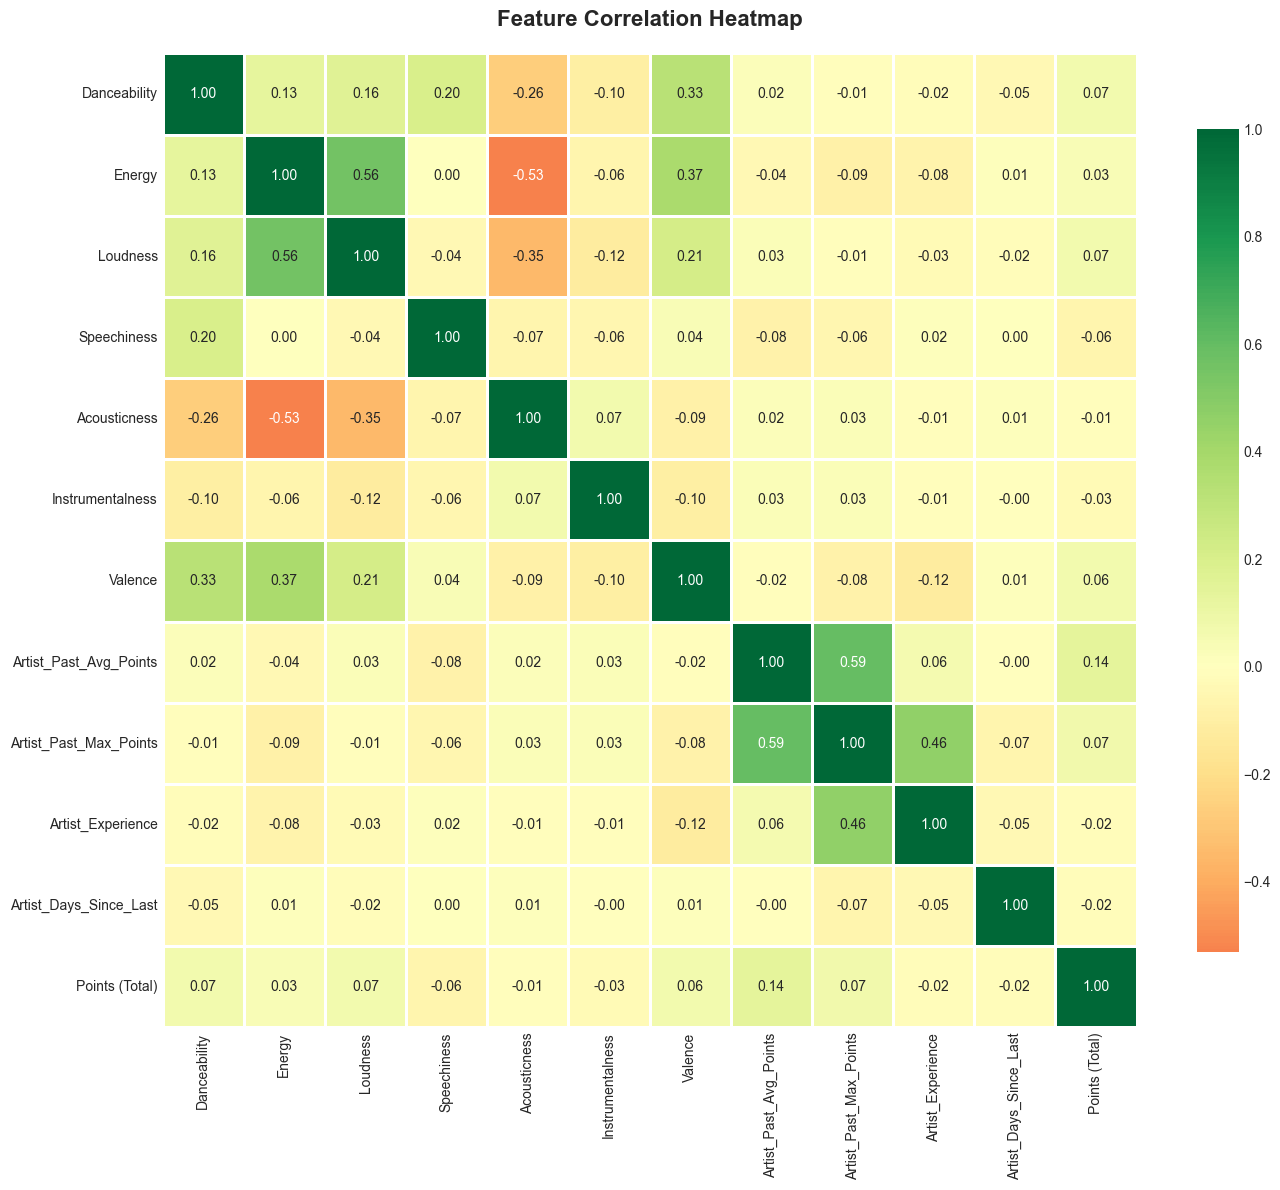
\includegraphics[height=0.6\textheight]{figs/correlation_matrix.png} % 60% of text height
\caption{Feature Correlation Heatmap}
\label{fig:correlation_heatmap}
\end{figure}


% ============ Monthly table ============ 
\begin{table}[h]
\centering
\resizebox{\textwidth}{!}{%
\begin{tabular}{|c|c|c|c|c|c|c|c|c|c|c|c|c|}
\hline
\textbf{Month} & \textbf{Jan} & \textbf{Feb} & \textbf{Mar} & \textbf{Apr} & \textbf{May} & \textbf{Jun} & \textbf{Jul} & \textbf{Aug} & \textbf{Sep} & \textbf{Oct} & \textbf{Nov} & \textbf{Dec} \\ \hline
\textbf{Points} & 5.33M & 4.78M & 5.18M & 4.97M & 5.10M & 5.01M & 5.25M & 5.28M & 5.05M & 5.15M & 4.97M & 5.15M \\ \hline
\end{tabular}%
}
\vspace{0.2cm}
\caption{Monthly patterns}
\label{tab:monthly_patterns}
\end{table}

% ============ Weekly table ============
\begin{table}[h]
\begin{tabular}{|c|c|c|}
\hline
\textbf{Day} & \textbf{Total Points} & \textbf{Relative to Avg} \\ \hline
Monday & 8,694,074 & -0.5\% \\ \hline
Tuesday & 8,691,338 & -0.5\% \\ \hline
Wednesday & 8,706,934 & -0.3\% \\ \hline
Thursday & 8,729,148 & +0.0\% \\ \hline
Friday & 8,751,691 & +0.3\% \\ \hline
Saturday & 8,888,057 & +2.2\% \\ \hline
Sunday & 8,759,639 & +0.6\% \\ \hline
\end{tabular}
\centering
\vspace{0.2cm}
\caption{Weekend effect with Saturday peak streaming}
\label{tab:weekday_patterns}
\end{table}

% ============ Table 02 ============ 
\begin{table}[h!]
% \renewcommand{\arraystretch}{1.3}
\begin{tabular}{p{3cm} p{9cm}}
\toprule
\textbf{Model} & \textbf{Hyperparameters (Search Space, with Optimal in Bold)} \\ \midrule

\textbf{Logistic Regression} &
\texttt{multi\_class}: '\textbf{multinomial}' \newline
\texttt{solver}: ['liblinear', 'saga', \textbf{lbfgs}] \newline
\texttt{max\_iter}: [\textbf{1000}] \newline
\texttt{class\_weight}: [\textbf{'balanced'}, None]
\\ \midrule

\textbf{Random Forest} &
\texttt{n\_estimators}: [\textbf{100}, 200, 300] \newline
\texttt{max\_depth}: [5, \textbf{10}, 20, None] \newline
\texttt{class\_weight}: [\textbf{'balanced'}, 'balanced\_subsample', None]
\\ \midrule

\textbf{XGBoost} &
\texttt{n\_estimators}: [\textbf{100}, 200, 300] \newline
\texttt{learning\_rate}: [0.01, \textbf{0.1}, 0.2] \newline
\texttt{max\_depth}: [3, 4, 5, \textbf{6}, 7] 
\\ \midrule

\textbf{SVM} &
\texttt{C}: \textbf{1.0} \newline
\texttt{kernel}: ['linear', '\textbf{rbf}', 'poly', 'sigmoid'] \newline
\texttt{gamma}: ['\textbf{scale}', 'auto', 0.001, 0.01, 0.1] \newline
\texttt{class\_weight}: ['\textbf{balanced}', None]
\\ \bottomrule

\end{tabular}
\centering
\caption{Hyperparameter search space and optimal hyperparameters for each model.}
\label{tab: Hyperparameter_search_space_for_models}
\end{table}

\end{appendices}
\end{document}